\documentclass[a4paper,12pt, oneside]{book}

%  Русский язык
\usepackage{cmap}					% Улучшенный поиск русских слов
\usepackage[T2A]{fontenc}			% кодировка
\usepackage[utf8]{inputenc}			% кодировка исходного текста
\usepackage[english,russian]{babel}	% локализация и переносы
\usepackage{pscyr}					% нормальные шрифты

% Колонтитулы
\usepackage{fancybox,fancyhdr}
\usepackage{lastpage}
\fancyhf{}
\fancypagestyle{all}
{
	\fancyhead{}
	\fancyhead[C]{\vspace{-5mm}Контрольная работа 12 Вариант Попов Юрий СКБ-171\vspace{3mm}}
	\fancyfoot{}
	\fancyfoot[C]{\hfill  \thepage  \hfill}
}

% Картинки и графики
\usepackage{wrapfig}
\usepackage{pgfplots}
\pgfplotsset{compat=1.9}

% Ссылки
\usepackage{xcolor}
\usepackage{color,colortbl} % раскраска таблиц
\usepackage[unicode, pdftex]{hyperref}
\definecolor{linkcolor}{HTML}{000000} 	% цвет ссылок
\definecolor{urlcolor}{HTML}{8B000F}	% цвет гиперссылок
\hypersetup{urlcolor=urlcolor, linkcolor=linkcolor, colorlinks=true}

% Размеры
\setlength{\paperwidth}{210mm}
\setlength{\paperheight}{297mm}
\setlength{\textheight}{225mm} 			% высота без колонтитулов
\setlength{\textwidth}{170mm}			% ширина текста
\oddsidemargin=0pt
\setlength{\headheight}{2mm}			% высота колонтитула
\setlength{\headsep}{5mm} 	% от блока текста до верхнего колонтитула
\setlength{\footskip}{10mm}  % от блока текста до нижнего колонтитула

% Математика
\usepackage{amsmath,amsfonts,amssymb,amsthm,mathtools,mathtext} 
\usepackage{latexsym,array,epsfig,wasysym}
\usepackage[all]{xy}
\let\int\varint
\def\Int{\int\limits}
\def\IInt{\iint\limits}
\def\IIInt{\iiint\limits}
\DeclarePairedDelimiter\floor{\lfloor}{\rfloor}


% Оглавление 
\usepackage{setspace}

\usepackage{tocloft} %регулировка расположения TableOfContent (Оглавления) на странице

%\setcounter{tocdepth}{1} % отменяет вывод в оглавление subsection and subsubsection
%\setcounter{secnumdepth}{1} %отменяет номерацию секций в тексте и оглавлении.
\usepackage{tocloft} %регулировка расположения TableOfContent (Оглавления) на странице

\renewcommand{\cfttoctitlefont}{\hspace{0.38\textwidth} \bfseries\MakeUppercase} %уменьшаем размер шрифта и ровняем по центру

% % Межстрочные отступы в Оглавлении:
\setlength{\cftbeforetoctitleskip}{5mm} %отступ Оглавления от верхнего поля страницы.
\setlength{\cftbeforechapskip}{14mm} %отступ между главами
\setlength{\cftbeforesecskip}{5mm} %отступ между секциями \section{title}

% % Отступы от левого поля:
\setlength{\cftchapindent}{1mm} %отступ между левым полем и \chapter{}
\setlength{\cftsecindent}{13mm} %отступ между левым полем и \section{title}

% % Отточия в Оглавлении
\renewcommand\cftchapdotsep{\cftdot} %добавляет отточия после \chapter{title}
%\renewcommand{\cftchapleader}{\cftdotfill{\cftchapdotsep}} %делает отточия после \chapter{title} тонкими, (по умолчанию жирные).
\renewcommand\cftsecdotsep{\cftdot} %делает отточия после \section{title} частыми.

% % Интервалы между абзацами, главами и так далее:
\usepackage{titlesec}

\titleformat{\chapter}[display]
{\filcenter}
{\MakeUppercase{\chaptertitlename} \thechapter}
{8pt}
{\bfseries}{}

\titleformat{\section}
{\normalsize\bfseries}
{\thesection}
{1em}{}

\titleformat{\subsection}
{\normalsize\bfseries}
{\thesubsection}
{1em}{}

% Настройка вертикальных и горизонтальных отступов
\titlespacing*{\chapter}{0pt}{-30pt}{8pt}
\titlespacing*{\section}{\parindent}{*4}{*4}
\titlespacing*{\subsection}{\parindent}{*4}{*4}


\begin{document} % начало документа	
\pagestyle{plain}

\begin{titlepage}	
	\begin{center}
		{\Huge \textbf{Математическая статистика}}
		\vspace{\baselineskip}
		
		{\huge Домашняя работа № 1 \\}
		\vspace{\baselineskip}
		{\huge Вероятностные распределения}
		\vspace{\baselineskip}
		
		{\large Попов Юрий, СКБ-172}
	\end{center}
\end{titlepage}



\begin{spacing}{0.99}          
	\tableofcontents %Оглавление. Корректно создается за два прогона tex файла.               
\end{spacing}

\newpage
Все графики, которые в дальнейшем будут вставлены в эту работу, были сконструированы с помощью библиотеки matplotlib в Jupyter Notebook, который будет приложен вместе с работой (Mathematical statistics $DZO$.ipynb)

\vspace{5mm}

Все определения были взяты из книги Зубкова А.М. "Учебное пособие по теории вероятностей и теории случайных процессов"


\vspace{13mm}%Задача 1
\textit{\textbf{Задание 1.1} Выбор одного дискретного распределения и одного непрерывного распределения}
\addcontentsline{toc}{chapter}{Задание 1.1 Выбор распределений}


\vspace{13mm}




Из представленных в задании таблиц я выбрал \textbf{Геометрическое} (дискретное) и \textbf{Экспоненциальное}(непрерывное) распределения

\vspace{\baselineskip}
\newpage
\vspace{13mm}%Задача 2
\textit{\textbf{Задание 1.2} Описание основных характеристик распределения}
\addcontentsline{toc}{chapter}{Задание 1.2 Описание основных характеристик распределения}
\\

\text{\large{\textbf {1.2.1 Экспоненциальное распределение}}}\\
\addcontentsline{toc}{section}{1.2.1 Экспоненциальное распределение}
\vspace{5mm}

	Пусть случайная величина задается законом распределения:
	$$
	f(x) = \lambda \exp(-\lambda x), x \in R, x > 0
	$$
	
	
	
	
	\vspace{5mm}
	\large{\textbf{Математическое ожидание}}
	\vspace{5mm}
	
	\normalsize{\textbf{Определение 1}} \textit{ Математическое ожидание} абсолютно непрерывной случайной величины $\xi$, распределение которой задаётся плотностью $f_x(x)$, равно
	$$
	E\xi = \int\limits_{-\infty}^{\infty} x f_x(x)dx
	$$
	
	Будем искать мат.ожидание через метод моментов.
	
	\vspace{\baselineskip}
	Найдем первый момент:
	$$
	M\xi = \int_0^\infty x f(x) dx = \int_0^\infty x \lambda \exp(-\lambda x)dx = [- x \exp(- \lambda x)]_0^\infty + \int_0^\infty \exp(-\lambda x) dx = \frac{1}{\lambda}
	$$
	Первый момент равен математическому  ожиданию, следовательно 
	$$
	 E\xi = \frac{1}{\lambda}
	$$	
	
	\vspace{5mm}
	\large{\textbf{Дисперсия}}
	\vspace{5mm}
	
	\normalsize{\textbf{Определение 2}} \textit{ Дисперсией } случайной величины называют математическое ожидание квадрата отклонения случайной величины от её математического ожидания
	$$
	D\xi = E(\xi - E(\xi))^2
	$$
	
	\vspace{\baselineskip}
	Будем искать дисперсию также через метод моментов.
	
	Найдем второй момент:
	
	$$
	M^2\xi = \int_0^\infty x^2 \lambda \exp(-\lambda x) dx = [-x^2 \exp(-\lambda x)]_0^\infty +\int_0^\infty 2 x \exp(-\lambda x)dx =
	$$ 
	
	$$
	= 0 + [-\frac{2}{\lambda} x \exp(-\lambda x)]_0^\infty + \int_0^\infty \exp(-\lambda x)dx = \frac{2}{\lambda}
	$$
	
	\vspace{\baselineskip}
	Определение можно записать по-другому:$D(X) = E(\xi^2) - E(\xi)^2$\\
	
	
	Соответственно, $D(X) = \frac{2}{\lambda} - \frac{1}{\lambda} = \frac{1}{\lambda}$ 
	\vspace{\baselineskip}
	
	Дисперсия равна:
	$$
	D\xi =  \frac{1}{\lambda}
	$$
	
	
	\vspace{5mm}
	\large{\textbf{Производящая функция моментов}}
	\vspace{5mm}
	
	\normalsize{\textbf{Определение 3}} Если случайная величина $X$ абсолютно непрерывна, то есть она имеет плотность $f_x(x))$, то \textit{ Производящая функция моментов } равна
		
	$$
	M_x(t) =  \int_{-\infty}^{+\infty} \exp(tx) f_x(x)dx
	$$
	
	\vspace{\baselineskip}
	Найдем производящую функцию моментов:
	
	$$
	\begin{array}{rcl}
	M_x(t) &=& E[\exp(tX)] \\
	\\
	&=& \int\limits_{-\infty}^{+\infty} \exp(tx) f_x(x)dx \\
	\\
	&=& \int\limits_0^\infty \exp(tx) \lambda \exp(-\lambda x)dx\\
	\\
	&=& \lambda \int\limits_0^\infty \exp((t-\lambda) x)dx\\
	\\
	&=&\lambda[\frac{1}{t-\lambda} \exp((t-\lambda) x)]_0^\infty\\
	\\
	&=&\frac{\lambda}{\lambda-t}
	\end{array}
	$$
	\\
	Производящая функция моментов:
	$$
	M_x(t) = \frac{\lambda}{\lambda-t}
	$$
	 
	 
	\newpage
	\large{\textbf{{Характеристическая функция}}}
	\vspace{5mm}
	
	\normalsize{\textbf{Определение 4}}\textit{ Характеристической функцией } случайной величины $\xi$ , принимающей действительные значения, называется функция 
	$$
	\varphi_x(t) = E[\exp(it\xi)],   \quad    -\infty <t < +\infty
	$$
	 
	\vspace{\baselineskip}
	Найдем характеристическую функцию:
	
	$$
	\begin{array}{rcl}
	\varphi_x(t) &=& E[\exp(itX)]\\
	\\
	&=&\int\limits_{-\infty}^{+\infty} \exp(itx) f_x(x)dx\\
	\\
	&=&\int\limits_0^\infty \exp(itx) \lambda \exp(-\lambda x)dx\\
	\\
	&=&\lambda \int\limits_0^\infty \cos(tx)\exp(-\lambda x)dx + i\lambda \int\limits_0^\infty \sin(tx)\exp(-\lambda x)dx
	\end{array}
	$$
	Отдельно посчитаем каждый интеграл:
	$$
	\begin{array}{rcl}
	\int\limits_0^\infty \cos(tx)\exp(-\lambda x)dx \\
	\\
	&=&[\frac{1}{t} \sin(tx) \exp(-\lambda x)]_0^\infty - \int\limits_0^\infty \frac{1}{t} \sin(tx)(-\lambda \exp(-\lambda x))dx\\
	\\
	&=&\frac{\lambda}{t} \int\limits_0^\infty \sin(tx) \exp(-\lambda x)dx\\
	\\
	&=&\frac{\lambda}{t}\{[-\frac{1}{t} \cos(tx) \exp(-\lambda x)]_0^\infty - \int\limits_0^\infty (-\frac{1}{t} \cos(tx))(-\lambda \exp(-\lambda x))dx\}\\
	\\
	&=&\frac{\lambda}{t}\left(\frac{1}{t} - \frac{\lambda}{t} \int\limits_0^\infty \cos(tx) \exp(-\lambda x)dx\right)\\
	\\
	&=&\frac{\lambda}{t^2} - \frac{\lambda ^2}{t^2} \int\limits_{0}^{\infty} \cos(tx) \exp(-\lambda x)dx
	\end{array}
	$$
	
	Получаем:
	$$
	\int\limits_0^\infty \cos(tx)\exp(-\lambda x)dx = \frac{\lambda}{t^2} - \frac{\lambda ^2}{t^2} \int\limits_{0}^{\infty} \cos(tx) \exp(-\lambda x)dx
	$$
	
	$$
	(1 + \frac{\lambda^2}{t^2})\int_0^\infty \cos(tx)\exp(-\lambda x)dx = \frac{\lambda}{t^2}
	$$
	
	$$
	\int\limits_0^\infty \cos(tx)\exp(-\lambda x)dx = \frac{\lambda}{(t^2 + \lambda^2)}
	$$
	
	Теперь считаем второй интеграл:
	$$
	\begin{array}{rcl}
	 \int\limits_0^\infty \sin(tx)\exp(-\lambda x)dx\\
	 \\
	 &=&[-\frac{1}{t} \cos(tx) \exp(-\lambda x)]_0^\infty- \int\limits_{0}^{\infty}(-\frac{1}{t} \cos(tx))(-\lambda \exp(-\lambda x))dx\\
	 \\
	 &=&\frac{1}{t} - \frac{\lambda}{t}\{ [\frac{1}{t} \sin(tx)\exp(-\lambda x)]_0^\infty - \int\limits_{0}^{\infty} \frac{1}{t} \sin(tx) (-\lambda \exp(-\lambda x ))dx  \}\\
	 \\
	 &=&\frac{1}{t} - \frac{\lambda}{t} (\frac{\lambda}{t} \int\limits_0^\infty \sin(tx) \exp(-\lambda x)dx)\\
	 \\
	  &=&\frac{1}{t} - \frac{\lambda ^2}{t^2} \int\limits_{0}^{\infty} \sin(tx) \exp(-\lambda x)dx
	 \end{array}
	$$
	
	Получаем:
	
	$$
	\int_0^\infty \sin(tx)\exp(-\lambda x)dx = \frac{1}{t} - \frac{\lambda ^2}{t^2} \int_{0}^{\infty} \sin(tx) \exp(-\lambda x)dx
	$$
	
	$$
	(1 + \frac{\lambda^2}{t^2}) \int_0^\infty \sin(tx)\exp(-\lambda x)dx = \frac{1}{t}
	$$
	
	$$
	\int_0^\infty \sin(tx)\exp(-\lambda x)dx = \frac{t}{t^2 + \lambda^2}
	$$

	Соединяем вместе:
	
	$$
	\begin{array}{rcl}
	\varphi_x(t) &=& \int\limits_0^\infty \cos(tx)\exp(-\lambda x)dx +  i \lambda \int\limits_0^\infty \sin(tx)\exp(-\lambda x)dx\\
	\\
	&=&\frac{\lambda^2}{(t^2 + \lambda^2)} + \frac{i\lambda t}{t^2 + \lambda^2}\\
	\\
	&=&\frac{\lambda}{\lambda - i t}
	\end{array}	
	$$
	
	\vspace{\baselineskip}
	Характеристическая функция:
	$$
	\varphi_x(t) = \frac{\lambda}{\lambda - i t}
	$$
	
	
	\vspace{5mm}
	\large{\textbf{{Функция распределения}}}
	\vspace{5mm}
	
	\normalsize{\textbf{Определение 5} Если случайная  величина $\xi$ , принимает действительные значения, то ее распределение удобно описывать  \textit{ функцией распределения }
	$$
		F_k(x) = P(k \le x), \quad -\infty < x < \infty
	$$
	
	
	\vspace{\baselineskip}
	Найдем функцию распределения:
	
	Если $x < 0$:(Потому что $x$ не может принимать отрицательные значения)
	$$
	F_x(x) = P(X \le x) = 0
	$$
	
	Если $x > 0$:
	$$
	\begin{array}{rcl}
	F_x(x) &=& P(X \le x)\\
	\\
	&=& \int\limits_{-\infty}^{x}f_x(t)dt\\
	\\
	&=& \int\limits_{0}^{x} \lambda\exp(-\lambda t)dt\\
	\\
	&=&[-\exp(-\lambda t)]_0^x\\
	\\
	&=&-\exp(-\lambda x) + 1
	\end{array}	
	$$
	
	Итого, получаем:
	

	\begin{equation*}
	F_x(x) = 
		\begin{cases}
			0 \text{	,$x < 0$}\\
			1 - \exp(-\lambda x) \text{		,$x \ge 0$}
		\end{cases}
	\end{equation*}
	

	\newpage
	\large{\textbf{{Графики}}}
	\vspace{5mm}	
			
	1)График плотности вероятности:

	\begin{minipage}[h]{0.55\linewidth}
		\center{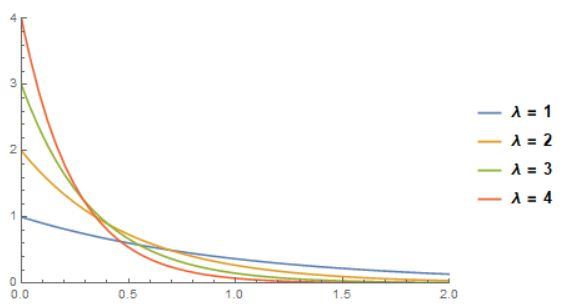
\includegraphics[width=1.5\linewidth]{graph_1.jpg} \\ Рис.1.2.1.1}
	\end{minipage}
	\\
	\vspace{\baselineskip}\\
	
	2)График функции распределения:\\
	\begin{minipage}[h]{0.55\linewidth}	
		\center{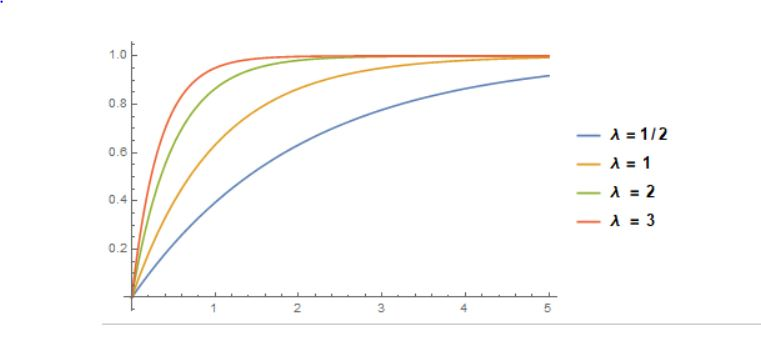
\includegraphics[width=1.5\linewidth]{graph_2.jpg} \\ Рис.1.2.1.2}
	\end{minipage}
	












\newpage	
\text{\large{\textbf {1.2.2 Геометрическое  распределение}}}\\
\addcontentsline{toc}{section}{1.2.2 Геометрическое распределение}
\vspace{5mm}


Пусть случайная величина задается законом распределения:
$$
p(x) =p (1 - p)^x, x \in N \bigcup \{0\}, 0 < p < 1
$$

\vspace{5mm}
\large{\textbf{Математическое ожидание}}
\vspace{5mm}

\normalsize{\textbf{Определение 6}} \textit{ Математическим ожиданием } неотрицательной дискретной случайной величины $\xi$ называется величина 
$$
E\xi = \sum\limits_{i=1}^\infty x_i p_i
$$

Будем искать мат.ожидание через метод моментов.


\vspace{\baselineskip}
Найдем первый момент:
$$
\begin{array}{rcl}
E[X] &=& \sum\limits_{x=0}^{\infty} (1-p)^x px \\
\\
&=&(1-p)p \sum\limits_{x=0}^{\infty} (1-p)^{x-1} x\\
\\
&=&-(1-p)p \sum\limits_{0}^{\infty} \frac{d}{dp} (1-p)^x\\
\\
&=&-(1-p)p \frac{d}{dp} \sum\limits_{0}^{\infty} (1-p)^x\\
\\
&=&-(1-p)p\frac{d}{dp} \frac{1}{1-(1-p)}\\
\\
&=&-(1-p)p\frac{d}{dp} \frac{1}{p}\\
\\
&=&-(1-p)p(-p^{-2})\\
\\
&=&(p-p^2)p^{-2}\\
\\
&=&\frac{1}{p} - 1\\
\\
&=& \frac{1-p}{p}
\end{array}
$$

Математическое ожидание:
$$
E[X] = \frac{1-p}{p}
$$



\vspace{5mm}
\large{\textbf{Дисперсия}}
\vspace{5mm}

\normalsize{\textbf{Определение 7}} \textit{ Дисперсией } случайной величины называют математическое ожидание квадрата отклонения случайной величины от её математического ожидания
$$
D\xi = E(\xi - E(\xi))^2
$$

Будем искать дисперсию также через метод моментов

Найдем второй момент:
$$
\begin{array}{rcl}
E[X^2] &=& \sum\limits_{0}^{\infty} (1 - p)^x px^2\\
\\
&=&(1-p)^2 p \sum\limits_{x=0}^{\infty} (1-p)^{x-2}x^2\\
\\
&=&(1-p)^2 p \sum\limits_{x=0}^{\infty} (1-p)^{x-2}x (x + 1 -1)\\
\\
&=&(1-p)^2 p \sum\limits_{x=0}^{\infty} (1-p)^{x-2}x (x -1) + \sum\limits_{x=0}^{\infty} (1-p)^{x}x \\
\\
&=&(1-p)^2 p  \sum\limits_{x=0}^{\infty} \frac{d^2}{dp^2}(1-p)^x + E[X]\\
\\
&=& (1-p)^2 p \frac{d^2}{dp^2} \sum\limits_{x=0}^{\infty} (1-p)^x + \frac{1-p}{p}\\
\\
&=&(1-p)^2 p \frac{d^2}{dp^2} \frac{1}{1-(1-p)} + \frac{1-p}{p}\\
\\
&=& (1-p)^2 p \frac{d^2}{dp^2} \frac{1}{p} + \frac{1-p}{p}\\
\\
&=& 2(1-p)^2 p\cdot p^{-3} + \frac{1-p}{p}\\
\\
&=&2(1-2p+p^2)p^{-2} + \frac{1-p}{p}\\
\\
&=&\frac{2 - 3p + p^2}{p^2}
\end{array}
$$

\vspace{\baselineskip}
Определение можно записать по-другому:$D(X) = E(\xi^2) - E(\xi)^2$\\

Соответственно,
$$
\begin{array}{rcl}
D(X) &=&\frac{2 - 3p+p^2}{p^2} - ({1-p}{p})^2\\
\\
&=&\frac{2-3p+p^2 -(1-2p + p^2)}{p^2}\\
\\
&=&\frac{1-p}{p^2}
\end{array}
$$

Итого, дисперсия равна 
$$
D(X) = \frac{1-p}{p^2}
$$



\vspace{5mm}
\large{\textbf{Производящая функция моментов}}
\vspace{5mm}

\normalsize{\textbf{Определение 8}} Если случайная величина $x$ дискретна, то есть она имеет плотность $P(X = x_i) = p_i$, то \textit{ Производящая функция моментов } равна

$$
M_x(t) =  \sum\limits_{i=1}^{\infty} \exp(tx_i) p_i
$$


Найдем производящую функцию моментов:

$$
\begin{array}{rcl}
M_x(t) &=& E[\exp(tX)] \\
\\
&=&\sum\limits_{0}^{\infty} (1 - p)^x p \exp(tx)\\
\\
&=& p \sum\limits_{0}^{\infty} [(1 - p)  \exp(t)]^x\\
\\
&=& \frac{p}{1-(1-p)\exp|(t)}
\end{array}
$$

\vspace{5mm}
Но у нас есть условие на t :
\vspace{3mm}

$(1 - p)  \exp(t) < 1 $
\vspace{3mm}

$\exp(t) < \frac{1}{1-p}$
\vspace{3mm}

$t < -\ln(1-p)$

\vspace{5mm}
Итого, производящая функция моментов геометрического распределения определена для $t < -\ln(1-p)$ и равна:
$$
M_x(t) = \frac{p}{1-(1-p)\exp|(t)}
$$


\newpage
\large{\textbf{{Характеристическая функция}}}
\vspace{5mm}

\normalsize{\textbf{Определение 9  }}Если случайная величина $x$ дискретна, то есть она имеет плотность $P(X = x_i) = p_i$, то \textit{ характеристическая функция } равна
$$
\varphi_x(t) =  \sum\limits_{i=1}^{\infty} \exp(tx_i) p_i
$$

Найдем характеристическую функцию:
$$
\begin{array}{rcl}
\varphi_x(t) &=& E[\exp(itX)]\\
\\
&=&\sum\limits_{0}^{\infty} (1-p)^x p \exp(itx)\\
\\
&=&p \sum\limits_{0}^{\infty} [(1-p)\exp(it)]^x\\
\\
&=&\frac{p}{1-(1-p)\exp(it)}
\end{array}
$$

Итого, характеристическая функция равна:
$$
\varphi_x(t) = \frac{p}{1-(1-p)\exp(it)}
$$


\normalsize{\textbf{Определение 10} Если случайная  величина $\xi$ , принимает действительные значения, то ее распределение удобно описывать  \textit{ функцией распределения }
$$
F_k(x) = P(k \le x), \quad -\infty < x < \infty
$$

\vspace{\baselineskip}
Найдем функцию распределения:

При $x < 0 : F_x(x) = 0$
При  $x > 0: $\\
$$
\begin{array}{rcl}
F_x(x) &=& P(X < x)\\
\\
&=&\sum\limits_{y=0}^x (1 - p)^y p\\
\\
&=&p \sum\limits_{y=0}^x (1 - p)^y\\
\\
&=&p \frac{1 - (1 - p)^{x + 1}}{1 - (1 - p)}\\
\\
&=& 1 - (1 - p)^{x + 1}
\end{array}
$$

Итого, функция распределения равна:
\begin{equation*}
F_x(x) = 
\begin{cases}
0 \text{	,    $x < 0$}\\
1 - (1 - p)^{x + 1} \text{		,      $x \ge 0$}
\end{cases}
\end{equation*}


\vspace{5mm}
\large{\textbf{{Графики}}}
\vspace{5mm}
	
1)Гистограмма вероятностей:

\begin{minipage}[h]{0.55\linewidth}
	\center{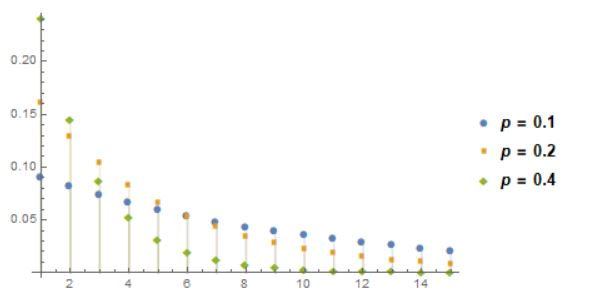
\includegraphics[width=1.5\linewidth]{graph_3.jpg} \\ Рис.1.2.3}
\end{minipage}
\\
\vspace{\baselineskip}\\

2)График функции распределения:\\
\begin{minipage}[h]{0.55\linewidth}	
	\center{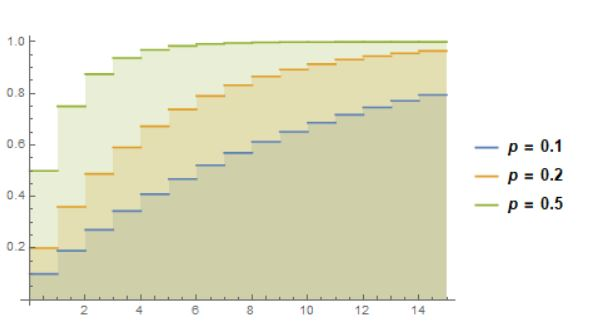
\includegraphics[width=1.5\linewidth]{graph_4.jpg} \\ Рис.1.2.4}
\end{minipage}









\newpage
\textit{\textbf{Задание 1.3} Поиск примеров событий, которые могут быть описаны выбранными случайными величинами}
\addcontentsline{toc}{chapter}{Задание 1.3 Поиск примеров событий}
\vspace{5mm}

\vspace{5mm}
\text{\Large{\textbf {1.3.1 Экспоненциальное распределение}}}\\
\addcontentsline{toc}{section}{1.3.1 Экспоненциальное распределение}
\vspace{5mm}

\vspace{5mm}
\text{\large{\textbf {1.3.1.1 Типичные интерпретации}}}\\
\addcontentsline{toc}{subsection}{1.3.1.1 Типичные интерпретации}
\vspace{5mm}

Экспоненциальное распределение оказывается весьма полезным в деловых приложениях, особенно при моделировании производства и систем массового обслуживания. 

Оно широко используется в теории расписаний (очередей) для моделирования промежутков времени между двумя запросами, которые могут представлять собой приход клиента в банк или ресторан быстрого обслуживания, поступление пациента в больницу, а также посещение Web-сайта.

В этой модели $\lambda $ - среднее количество запросов, поступающих в систему за единицу времени. 

Величина $1/\lambda $ равна среднему промежутку времени, прошедшего между двумя последовательными запросами.

И тогда  вероятность того, что следующий запрос поступит раньше, чем через X единиц времени, определяется по формуле:  $1- \exp(-\lambda x)$ 
\\


\vspace{5mm}
\text{\large{\textbf {1.3.1.2 Нетипичные интерпретации}}}\\
\addcontentsline{toc}{subsection}{1.3.1.2 Нетипичные интерпретации}
\vspace{5mm}

Экспоненциальное распределение активно используется в теории 

надежности.\cite{rt5}


Теория надёжности изучает методы обеспечения стабильности работы объектов (конструкций, изделий, устройств, систем и т. п.) в процессе проектирования, производства, приёмки, транспортировки, эксплуатации и хранения.

Экспоненциальный закон распределения называемый также основным законом надежности, часто используют для прогнозирования надежности в период нормальной эксплуатации изделий, когда постепенные отказы еще не проявились и надежность характеризуется внезапными отказами

Рассмотрим примеры неблагоприятного сочетания условий работы деталей машин,вызывающих их внезапный отказ. Для зубчатой передачи это может быть действием максимальной нагрузки на наиболее слабый зуб при его зацеплении;
для элементов радиоэлектронной аппаратуры — превышение допустимого тока или температурного режима.

Когда за случайную величину принимается время работы объекта t, вероятность того, что изделие на протяжении времени t будет находиться в работоспособном состоянии, равна
$$
P(t) = \exp(-\lambda t)
$$
,где $\lambda-$ интенсивность отказов объекта, а $t$ время работы объекта

\vspace{5mm}
\text{\large{\textbf {1.3.1.3 Известные соотношения}}}\\
\addcontentsline{toc}{subsection}{1.3.1.3 Известные соотношения}
\vspace{5mm}

{\sf$\bullet$ Связь с Гамма-распределением}
\vspace{5mm}

$$
Exp(\lambda) \equiv Г(1, 1/\lambda)
$$

\vspace{5mm}
{\sf$\bullet$ Связь с $\chi^2$}
\vspace{5mm}

$$
Exp(1/2) \equiv \chi^2(2)
$$

\vspace{5mm}
{\sf$\bullet$ Связь с одномерным непрерывным равномерным распределением}
\vspace{5mm}

Можно получить экспоненциальное распределение из  непрерывного равномерного распределения методом обратного преобразования. Пусть $U \sim U[0,1]$. Тогда
$$
X=-\frac{1}{\lambda}\ln U \sim Exp[\lambda]
$$

\vspace{5mm}
{\sf$\bullet$ Экспоненциальное распределение является частным случаем распределения Вейбулла}
\vspace{5mm}

Экспоненциальное распределение также является частным случаем распределения Вейбулла, которое происходит, когда параметр формы Вейбулла равен 1
 
\vspace{5mm}
{\sf$\bullet$ Связь с распределением Эрланга}
\vspace{5mm}

Время обслуживания агентов(например, сколько времени требуется сотруднику, чтобы обслужить клиента) также можно смоделировать как экспоненциально распределенные переменные.
Общая длина процесса ( последовательность из нескольких независимых задач) следует распределению Эрланга: распределение суммы нескольких независимых экспоненциально распределенных переменных

\vspace{5mm}
{\sf$\bullet$ Связь с распределением Пуассона}
\vspace{5mm}

Экспоненциальное распределение связано с распределением Пуассона. В то время как экспоненциальная модель моделирует время между последовательными событиями на непрерывном временном интервале, распределение Пуассона имеет дело с событиями, которые происходят в течение фиксированного периода времени

\vspace{5mm}
{\sf$\bullet$ Экспоненциальное распределение является распределением Пирсона типа X}
\vspace{5mm}

\vspace{5mm}
{\sf$\bullet$ Связь с геометрическим распределением}
\vspace{5mm}

Дискретный вариант экспоненциального распределения — это геометрическое распределение






\newpage
\text{\Large{\textbf {1.3.2 Геометрическое  распределение}}}\\
\addcontentsline{toc}{section}{1.3.2 Геометрическое распределение}
\vspace{5mm}

\vspace{5mm}
\text{\large{\textbf {1.3.2.1 Типичные интерпретации}}}\\
\addcontentsline{toc}{subsection}{1.3.2.1 Типичные интерпретации}
\vspace{5mm}

Геометрическое распределение часто используется в азартных настольных играх. В зависимости от вытащенной карты, или суммы брошенных кубиков игрок выигрывает или побеждает. Соответственно, считая вероятность в каждом раунде(при каждом броске) игрок увеличивает свои шансы на успех

\vspace{5mm}
\text{\large{\textbf {1.3.2.2 Нетипичные интерпретации}}}\\
\addcontentsline{toc}{subsection}{1.3.2.2 Нетипичные интерпретации}
\vspace{5mm}

Нетипичной интерпретацией использования геометрического распределения является использования его в генетике.\cite{rt4}

Предположим, мы анализируем последовательности ДНК ряда генов у некоторых видов. Возможно, нас  заинтересует химия, лежащая в основе этих генов, и мы захотим изучить конкретные последовательности нуклеотидов, которые имеют тенденцию происходить. В частности, предположим, что всякий раз, когда в гене присутствует Т-нуклеотид, нам хотелось бы разработать модель относительно количества нуклеотидов до следующего T. Рассмотрим следующую часть последовательности ДНК: 
$$
...AAGTGGGAGGCCATCCA.....
$$

Начинаем двигаться по ДНК...Как только мы столкнемся с первым T (тем, что находится в четвертой позиции), сколько времени пройдет, пока мы не столкнемся со следующим Т? Важно, что мы определяем успех как наличие T на определенной позиции. Это случайный процесс, и количество нуклеотидов - случайная величина. Это приведет к различному значению в зависимости от того, какой нуклеотид T является отправной точкой, какой ген мы выбрали и другие факторы. Для этой конкретной последовательности, мы наблюдали бы N = 10, так как наш первый успех (еще один T) произошел на 10-й позиции от начала. Затем можно было бы измерить количество нуклеотидов до следующего т после этого и рассмотрим еще одно наблюдение N.

Получается, что N -  случайная величина, а процесс нахождения нужного нам нуклеотида  подчиняется геометрическому распределению

\vspace{5mm}
\text{\large{\textbf {1.3.2.3 Известные соотношения}}}\\
\addcontentsline{toc}{subsection}{1.3.2.3 Известные соотношения}
\vspace{5mm}

{\sf$\bullet$ Связь с отрицательным биномиальным распределением }
\vspace{5mm}

Геометрическое распределение является частным случаем отрицательного биномиального распределения:
$$
Geom(p) \equiv NB(1,p)
$$

\vspace{5mm}
{\sf$\bullet$ Связь с экспоненциальным распределением }
\vspace{5mm}

Геометрическое распределение рассматривается как дискретный вариант экспоненциального распределения.\\

Предположим, что эксперименты Бернулли выполняются через равные промежутки времени. Тогда геометрическая случайная величина X - это время, измеренное в дискретных единицах, которое проходит до того, как мы получим первый успех. Но если мы хотим смоделировать время, прошедшее до того, как данное событие произошло в непрерывном времени, то подходящим распределением для использования является экспоненциальное распределение




\newpage
\textit{\textbf{Задание 1.4} Описание способа моделирования выбран-
	ных случайных величин}
\addcontentsline{toc}{chapter}{Задание 1.4 Моделирование}
\vspace{13mm}

\vspace{5mm}
\text{\Large{\textbf {1.4.1 Экспоненциальное распределение}}}\\
\addcontentsline{toc}{section}{1.4.1 Экспоненциальное распределение}
\vspace{5mm}


Составим программу моделирования случайной величины X.

Функция распределения имеет вид:
$$
F(x) = 1 - \exp(-\lambda x)
$$

Согласно методу обратных функций:\cite{rt1}
$$
F(x) = 1 - \exp(- \lambda x) = r
$$

Получим:
$$
\exp(- \lambda x) = 1 - r
$$

Таким образом:
$$
- \lambda x = \ln(1 - r)
$$

И

$$
x = -\frac{1}{\lambda} \ln(1 - r)
$$

Так как случайная величина $(1 - r)$ имеет такое же распределение, что и $r$, то при нахождение значений случайной величины X пользуемся формулой:
$$
x = - \frac{1}{\lambda} \ln r
$$

Соответственно, составляем программу для моделирования случайной величины.

Получаем такие результаты:

\begin{figure}[h]
	\begin{center}
		\begin{minipage}[h]{0.4\linewidth}
			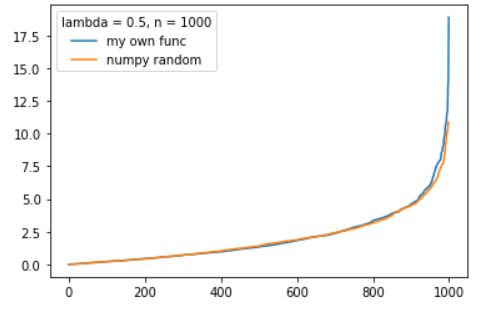
\includegraphics[width=1\linewidth]{ex_1_1000.jpg}
			\caption{n = 1000} %% подпись к рисунку
			\label{ris:experimoriginal} %% метка рисунка для ссылки на него
		\end{minipage}
		\hfill
		\begin{minipage}[h]{0.4\linewidth}
			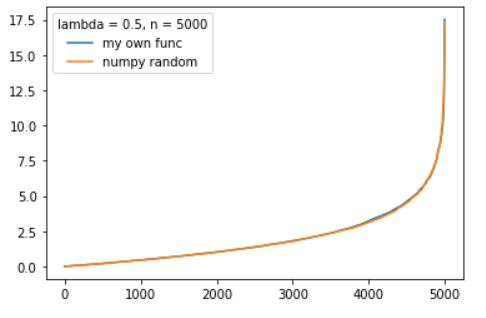
\includegraphics[width=1\linewidth]{ex_1_5000.jpg}
			\caption{n = 5000}
			\label{ris:experimcoded}
		\end{minipage}
	\end{center}
\end{figure} 

\begin{center}
	\begin{minipage}[h]{0.4\linewidth}
		\center{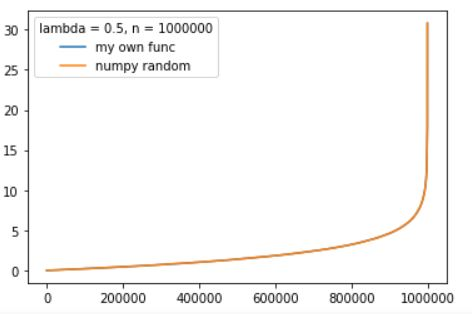
\includegraphics[width=1\linewidth]{ex_1_16.jpg} \\ Рис.3 n = 1000000}
	\end{minipage}
\end{center}


\vspace{5mm}
{\large{\bf Оценка времени}}
\vspace{5mm}

Ниже будет приведен код, который с помощью magic commands в Jupyter Notebook вычисляет работу отдельного куска кода. 

В первой ячейке идет расчет времени собственного способа моделирования. А во второй встроенной функции numpy

\vspace{5mm}
\begin{minipage}[h]{0.4\linewidth}
	\center{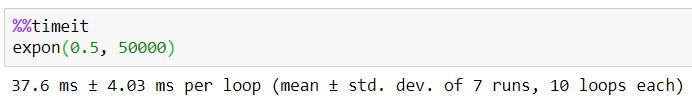
\includegraphics[width=2.5\linewidth]{ex_time_1.jpg} \\ }
\end{minipage}
\vspace{5mm}

\vspace{5mm}
\begin{minipage}[h]{0.4\linewidth}
	\center{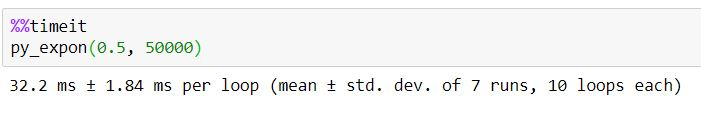
\includegraphics[width=2.5\linewidth]{ex_time_2.jpg} \\ }
\end{minipage}
\vspace{5mm}


По результат время моделирования приблизительно оказалось равно

\vspace{5mm}
\text{\Large{\textbf {1.4.2 Геометрическое  распределение}}}\\
\addcontentsline{toc}{section}{1.4.2 Геометрическое распределение}
\vspace{5mm}


Геометрическое распределение $Geom(p)$  с параметром $p \in (0,1)$ описывается с помощью бесконечной таблицы распределения:
$$
P: \left(
\begin{array}{cccccc}
0 & 1 & 2& 3 &\ldots & k\\
p_0 & p_1 & p_2 & p_3 & \ldots &  p_k
\end{array}
\right)
$$

где $p_k = p(1 - p)^k$

Есть два способа способа моделирования геометрического распределения.

Первый - моделирование испытаний Бернулли с вероятностью успеха  p до первого успеха с подсчетом числа неудач.

Второй - последовательный метод обратных функций, основанный на пересчете $p_n = (1 - p)p_{n-1}$ c $p_0 = p$

Смоделируем первый вариант:

\begin{figure}[h]
	\begin{center}
		\begin{minipage}[h]{0.4\linewidth}
			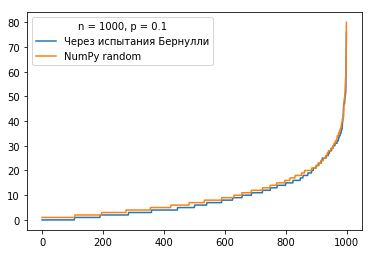
\includegraphics[width=1\linewidth]{py_1_1000.jpg}
			\caption{n = 1000} %% подпись к рисунку
			\label{ris:experimoriginal} %% метка рисунка для ссылки на него
		\end{minipage}
		\hfill
		\begin{minipage}[h]{0.4\linewidth}
			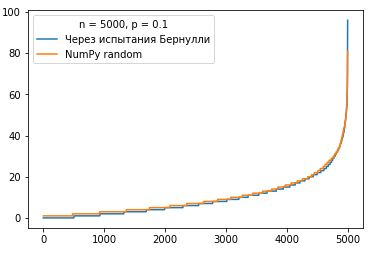
\includegraphics[width=1\linewidth]{py_1_5000.jpg}
			\caption{n = 5000}
			\label{ris:experimcoded}
		\end{minipage}
	\end{center}
\end{figure} 



\begin{center}
	\begin{minipage}[h]{0.4\linewidth}
		\center{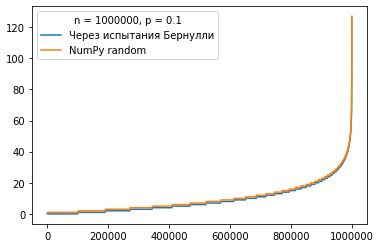
\includegraphics[width=1\linewidth]{py1_16.jpg} \\  n = 1000000}
	\end{minipage}
\end{center}


\vspace{15mm}
Теперь с помощью алгоритма метода обратных функций построим следующие распределения:

\begin{figure}[h]
	\begin{center}
		\begin{minipage}[h]{0.4\linewidth}
			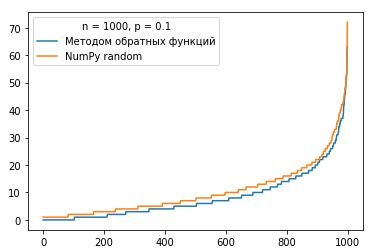
\includegraphics[width=1\linewidth]{py_2_1000.jpg}
			\caption{n = 1000} %% подпись к рисунку
			\label{ris:experimoriginal} %% метка рисунка для ссылки на него
		\end{minipage}
		\hfill
		\begin{minipage}[h]{0.4\linewidth}
			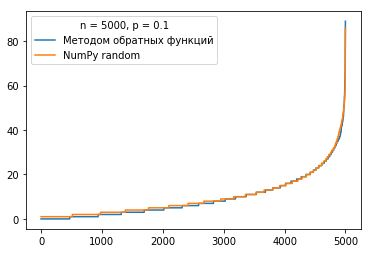
\includegraphics[width=1\linewidth]{py_2_5000.jpg}
			\caption{n = 5000}
			\label{ris:experimcoded}
		\end{minipage}
	\end{center}
\end{figure} 


\begin{center}
	\begin{minipage}[h]{0.4\linewidth}
		\center{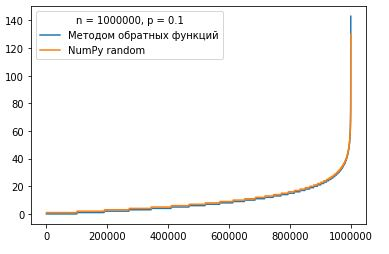
\includegraphics[width=1\linewidth]{py_2_16.jpg} \\ n = 1000000}
	\end{minipage}
\end{center}


\vspace{15mm}
Первые два метода плохи при малых p. Существует однако такой способ реализации метода обратных функций, при котором трудоемкость по крайней мере формально не зависит от p
Теперь с помощью модифицированного прямого метода обратных функций построим следующие распределения:

\begin{figure}[h]
	\begin{center}
		\begin{minipage}[h]{0.4\linewidth}
			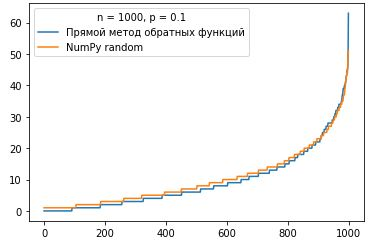
\includegraphics[width=1\linewidth]{py_3_1000.jpg}
			\caption{n = 1000} %% подпись к рисунку
			\label{ris:experimoriginal} %% метка рисунка для ссылки на него
		\end{minipage}
		\hfill
		\begin{minipage}[h]{0.4\linewidth}
			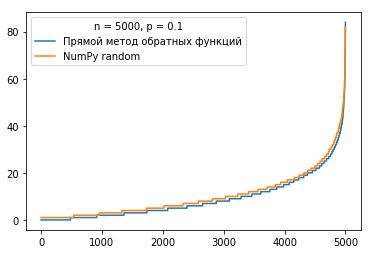
\includegraphics[width=1\linewidth]{py_3_5000.jpg}
			\caption{n = 5000}
			\label{ris:experimcoded}
		\end{minipage}
	\end{center}
\end{figure} 


\begin{center}
	\begin{minipage}[h]{0.4\linewidth}
		\center{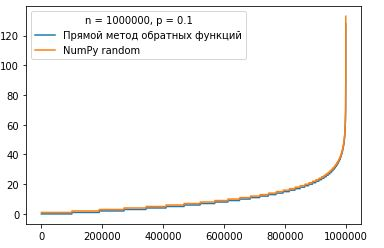
\includegraphics[width=1\linewidth]{py_3_16.jpg} \\ n = 1000000}
	\end{minipage}
\end{center}



Для моделирования геометрического распределения третьим методом  требуется одно обращение к генератору псевдослучайных чисел, два вычисления логарифма и одно — целой части числа. Если считать, что время вычисления значений функций $ \floor*{x}$ и  $\ln(z)$ ограничено при всех $x, z \in (0,1)$ одно	 и той же постоянной, то трудоемкость алгоритма имеет вид О(1) равномерно по p 

\vspace{5mm}
{\large{\bf Оценка времени}}
\vspace{5mm}

Ниже будет приведен код, который с помощью magic commands в Jupyter Notebook вычисляет работу отдельного куска кода. 

По порядку в четырёх ячейках представлены время работы каждого метода, а также время работы встроенной  функции.

\vspace{5mm}
\begin{minipage}[h]{0.4\linewidth}
	\center{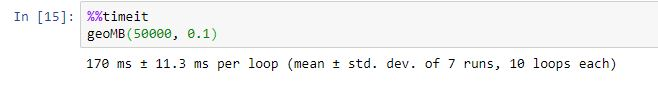
\includegraphics[width=2.5\linewidth]{time_1.jpg} \\ }
\end{minipage}
\vspace{5mm}

\vspace{5mm}
\begin{minipage}[h]{0.4\linewidth}
	\center{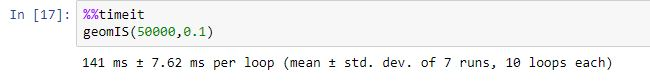
\includegraphics[width=2.5\linewidth]{time_2.jpg} \\ }
\end{minipage}
\vspace{5mm}

\vspace{5mm}
\begin{minipage}[h]{0.4\linewidth}
	\center{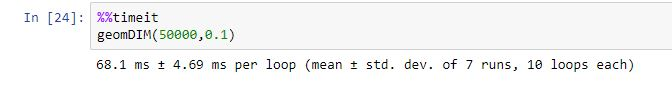
\includegraphics[width=2.5\linewidth]{time_3.jpg} \\ }
\end{minipage}
\vspace{5mm}

\vspace{5mm}
\begin{minipage}[h]{0.4\linewidth}
	\center{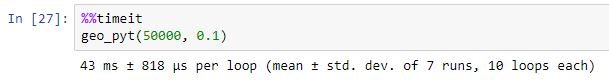
\includegraphics[width=2.5\linewidth]{time_4.jpg} \\ }
\end{minipage}
\vspace{5mm}


Как видно из рисунков, реализация библиотечной функции примерно в 400 раз быстрее первого метода.
\begin{thebibliography}{99}
	\bibitem{rt1} В.В Некруткин "Моделирование распределений"
	\bibitem{rt2} Medium // \href{https://towardsdatascience.com/what-is-exponential-distribution-7bdd08590e2a}{ссылка1}
	\bibitem{rt3} Statistics // \href{https://www.statisticshowto.datasciencecentral.com/exponential-distribution/}{ссылка2}
	\bibitem{rt4} Paul Maiste Probablity and Statistics for Bioinformatics and Genetics // \href{http://www.ams.jhu.edu/~dan/550.435/notes/COURSENOTES435.pdf}{ссылка3}
	\bibitem{rt5} Теория надежности // \href{http://www.obzh.ru/nad/4-3.html}{ссылка4}
\end{thebibliography}

\end{document}
